\documentclass{school-22.211-notes}
\date{February 22, 2012}

\begin{document}
\maketitle


\clearpage
\topic{Resonance Integrals vs. Group Cross Section}
We introduce \hi{(Infinite) Resonance Integrals} as flux weighted (that is, weighted with 1/E spectrum $\phi(E) \sim \frac{1}{E}$) microscopic cross section: 
\begin{align}
\RI &=  - \int_{u1}^{u2} \sigma(u) \du \\
u &= \ln \left( \frac{E_0}{E} \right) = \ln(E_0) - \ln E \\
\du &= - \frac{1}{E} \dE \\ 
\RI &=  \int \sigma (E) \frac{1}{E} \dE 
\end{align}
Notice, 
\begin{itemize}
\item RI is defined directly from cross section data; no flux calculation is required because 1/E spectrum is assumed; 
\item RI depends on the normalization of the 1/E flux spectrum; it is also implicitly assumed that flux equals 1 when $E = 1$ through normalization;
\item RI is independent of energy bounds for isolated resonances;
\item RI is independent of temperature. This is because if the energy bound is larger enough, then as temperature increases, the spectrum would broaden, but because the area under the curve remains the same, assume the cross section is constant, then RI is essentially integrating the spectrum, which would not change upon temperature change;
\item RI is useful for inter-comparing libraries or cross section models. It is a classic way to evaluate new resonance data typically from 0.5 eV to 10 keV. We use RI to check our resonance data, in particularly the three big resonances at 6.67, 21, 26 eV. Numerical test of the SLBW RIs shows that the RI comes out to be within 1\% of ENDF/B-VII Reich-Moore data (Lec 6, slide 17, with 0.01 eV as spacing in histogram). 
\end{itemize}

\hi{Group cross section} is a similar but much more useful quantity. From its definition, we see $\sigma_g$ does not depend on the flux normalization: 
\begin{align}
\sigma_g &= \frac{\int_{E_1}^{E_2} \sigma(E) \phi(E) \dE }{\int_{E_1}^{E_2} \phi(E) \dE} 
\end{align}
If we make assumptions on the flux spectrum, then we can relate $\sigma_g$ to $\RI_{\eff}$,
\begin{align}
\phi(E) &\sim \frac{1}{E} \\
\sigma_g &= \frac{\int_{E_1}^{E_2} \sigma(E) \frac{1}{E} \dE }{\int_{E_1}^{E_2} \frac{1}{E} \dE} 
= \frac{\RI_{\eff}}{\ln(E_2) - \ln(E_1)}  
= \frac{\RI_{\eff}}{\ln(E_2/E_1)} \\
\Aboxed{\RI_{\eff} &= \sigma_g \ln(E_2/E_1) } \label{RIeff}
\end{align}
Notice\footnote{Review here for exam}:
\begin{itemize}
\item Group cross section by definition depends on both cross section and flux spectrum. 
\item Group cross section depends on the flux, but not on the normalization of flux (that is, only the shape matters, not the magnitude);
\item Group cross section depend explicitly on energy bounds (widths) of the groups; 
\item Effective RI can be computed from group cross sections and group energy bounds as in Eq.~\ref{RIeff}; As spectrum approaches 1/E, the effective RI computed from group cross sections will approach infinite RI. 
\end{itemize}


\clearpage
%%%%%%%%%%%%%%%%%%%%%% Doppler Broadening %%%%%%%%%%%%%%%%%%
\topic{Doppler Broadening/Temperature Effects On Cross Section}
\hi{Doppler Broadening} means, as the temperature increases, the width of the spectrum decreases, although the area under the curve stays the same\footnote{References: Reuss Section 8.4; Handbook of Nuclear Engineering Chapter 4 Section 3; Duderstadt p.337-338; Bell p.433 (points out the area under the cross section curve is constant; hence the absorption rate is proportional to the magnitude of the flux in a sense.)}. 
There are two possibilities: 
\begin{enumerate}
\item Infinite RI (infinite dilution factor, negligible absorber concentration, $\Sigma_t \sim \Sigma_s^M$) is independent of temperature becase the area under the psi chi curves are constant. The absorber concentration is too low to perturb the flux, hence no flux depression and no self-shielding.  
\item Effective RI (finite concentration of \ce{^{238} U}) is dependent of temperature and the resonant material density because of the energy self-shielding effect as in Figure~\ref{Doppler}: 
  \begin{itemize}
  \item If temperature increases, $\RI_{\eff}$ would increase, because the broadened resonance increases the energy range over which abosrption occurs, which outweighs the lowering of the resonance peak. Reason: Energy self-shielding (the strong absorption of the resonance tends to shield the absorber nucleir from neutrons with energy $E\sim E_0$, hence the term `flux depression').  As temperature increases, the resonance is broadened by the Doppler effect, the neutron flux depression is decreased, whereas the area under the cross section curve is essentially constant. Hence the resonance absorption which is the energy-integrated reaction rate $\Sigma_a(E) \phi(E)$ increases with increasing temperature. 
  \item If U/H increases, there are two consequences: one is that the flux is more depressed hence the $\RIeff$ decreases; secondly the higher energies become more important as we would later see in Section~\ref{spectral-hardening-section}. 
  \item \textit{The higher the concentration of U238, the larger the Doppler temperature effects become.}
  \end{itemize}
\end{enumerate}


\textbf{Why do resonance broaden?} 

If a neutron's energy equals that of the resonance, it will be absorbed. If it is
slightly above or below the resonance energy, it will scatter off the U-238 nuclei
without absorption. As the fuel heats up, the nuclei vibrate and this changes the
relative speed between the neutron and the nuclei. Hence, the neutron is
effectively at a different energy. What are the consequences? Suppose a neutron
is initially slightly below the resonance energy. If the nucleus moves toward the
neutron, the relative speed between the two goes up. Hence, that neutron will be
absorbed.

But for every neutron that is now newly absorbed, one that was previously at the
resonance energy is now too high and it only scatters off the nucleus. So, why is
there a net increase in absorption? The reason is that scattered neutron loses only
a slight amount of energy (small object bouncing off a large one) and on its next
collision, which will likely be with the fuel again, it will be absorbed. Thus, U-
238 resonances broaden because (1) the U-238 nuclei vibrate more rapidly on heat
up and (2) the fuel is separate from the coolant so that successive interactions
occur in the fuel.

\begin{figure}
  \begin{subfigure}[b]{0.45\textwidth}
    \centering
    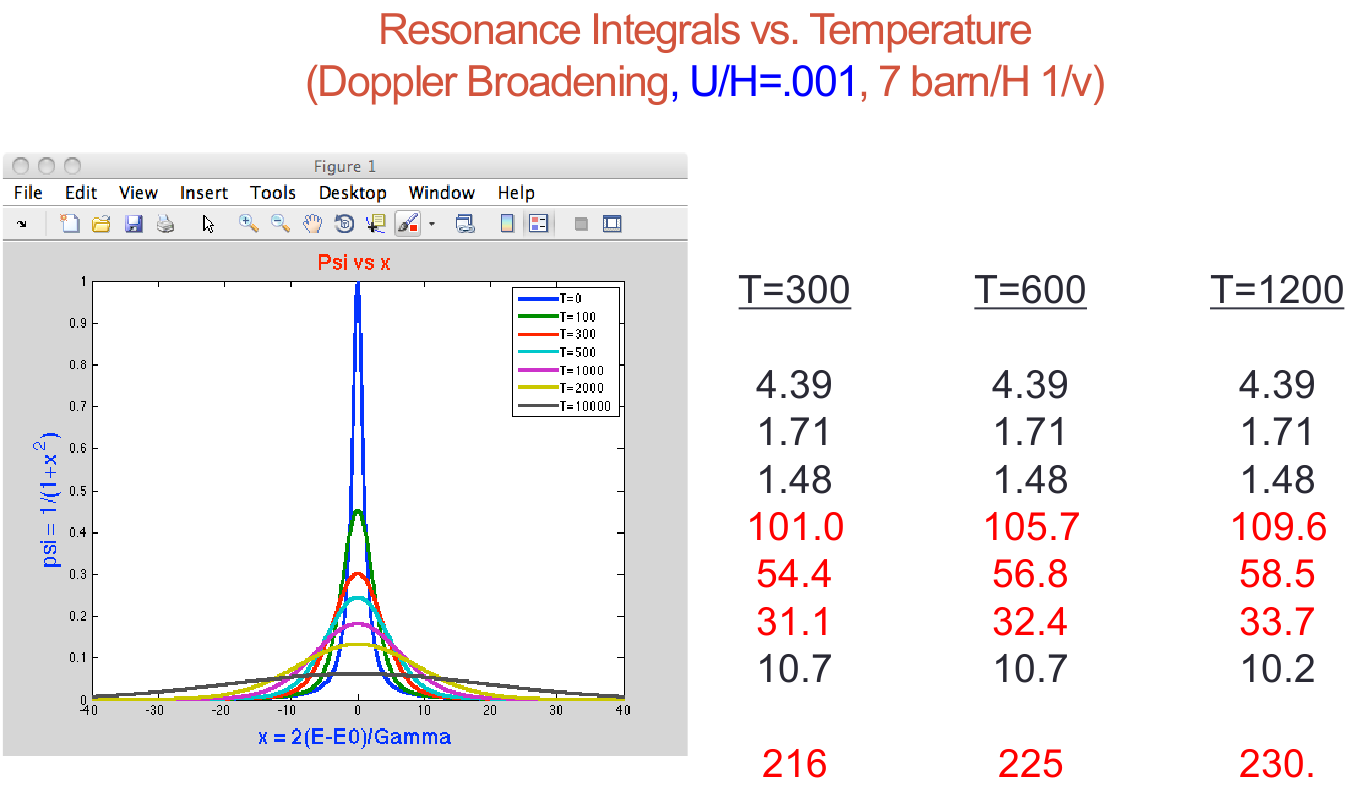
\includegraphics[width=\textwidth]{images/r-m/Doppler-RI-1.png}
    \caption{U/H = 0.001} \label{UH0.01}
  \end{subfigure}
  \begin{subfigure}[b]{0.45\textwidth}
    \centering
    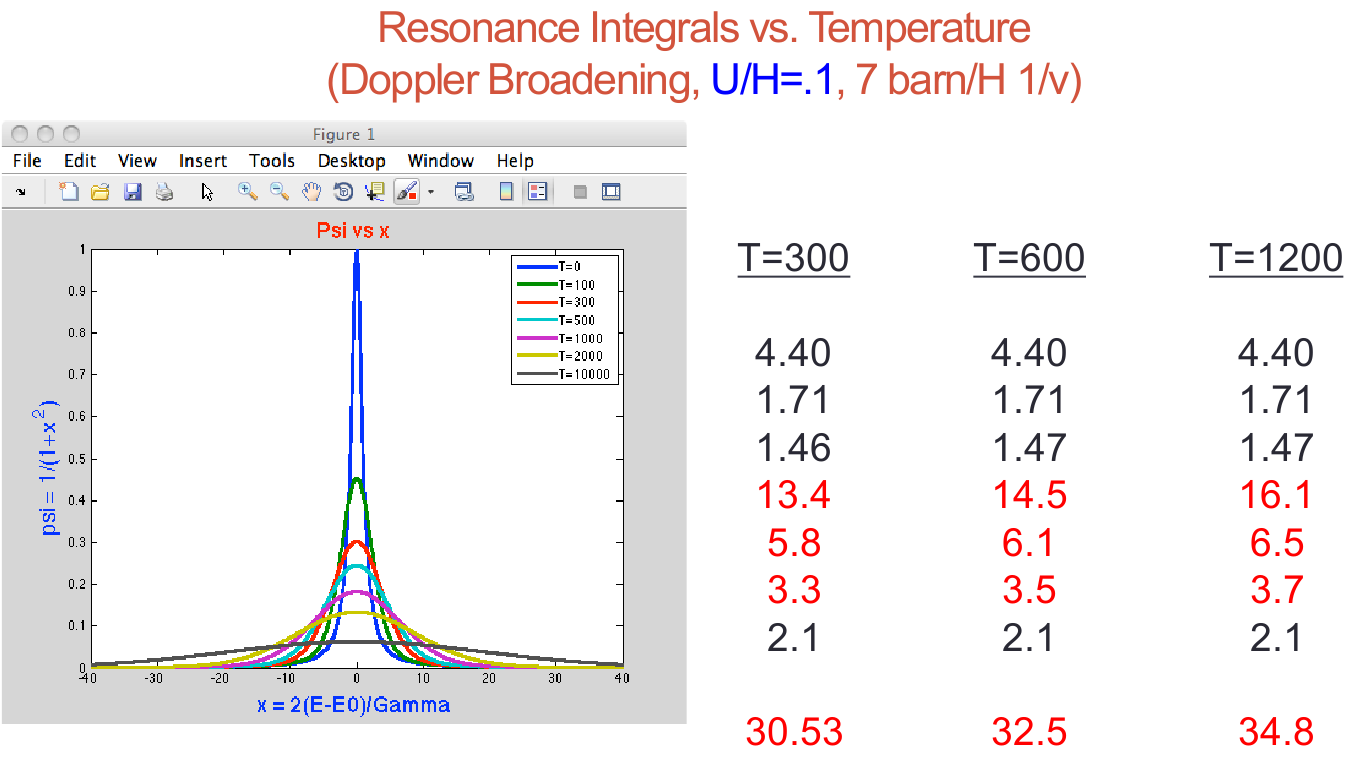
\includegraphics[width=\textwidth]{images/r-m/Doppler-RI-2.png}
    \caption{U/H = 0.1} \label{UH0.1}
  \end{subfigure}
  \caption{Impact of Temperature On Effective RI, Doppler Broadening} \label{Doppler}
\end{figure}


\clearpage
%%%%%%%%%%%%%%%%%%% SELF-SHIELDING %%%%%%%%%%%%%%%%%%%%%
\topic{Self-Shielding Effects On Spectrum}
Self-shielding/flux depression is first observed through: 
\begin{table}[ht]
  \centering
  \begin{tabular}{|l|p{6cm}|p{6cm}|} \hline
    & Observation & Explaination \\ \hline
    Spatial 
    & if natural uranium was made into a lump surrounded by moderator, resonance absorption $\down \down$  
    & U238 in the center of a pin is `shielded' from neutrons in the moderator \\ \hline
    Energy
    & if U/H $\up$, absorption rate per atom (for neutrons slowed down in a water \& U mix) $\down$   
    & the magnitude of absorption is proportional to the width of the resonance;  \\ \hline
  \end{tabular}
  \caption{Observation Concerning Self-Shielding}
  \end{table}

\subtopic{Spatial self-shielding} 
In a sentence, lumped configuration shields the fuel region from neutrons with $E \sim E_0$, hence decreasing resonance absorption and increasing $p$. As fuel diameter increases, the RI -- and therefore the absorption -- decreases. 

For a homogenized medium, the value of p for natural uranium is about 0.70.
However, larger values exist for the heterogeneous case. This is because of a
phenomenon called ``spatial self-shielding.'' The idea is to keep the fuel and
moderator separate. Neutrons slow down in a stepwise manner. Some collisions
will cause neutrons to jump over the energies that correspond to the U238
resonances. Others will land in resonance energies. What happens to these neutrons? 
Suppose a neutron has an energy close to that of a U-238 resonance. 
\begin{itemize}
\item If a neutron scatters off U238 it will lose
only a small amount of energy. In this case, the neutron is
left near the resonance energy.
\item If it scatters off moderator it will lose a lot of its energy.  In this case the neutron is removed from that energy.
\end{itemize}

What then is the effect of homogeneous or heterogeneous fuel? If the fuel and
moderator are separate and the neutron is in the moderator, chances are it will
collide with another moderator atom and be scattered out of the resonance region.
So, heterogeneous arrangements favor resonance escape. In contrast, if the fuel
and moderator are infinitely mixed (homogeneous) or if the fuel rod/moderator
volumes repeat on small scales with dimensions less than a diffusion length, the
next collision may again be with fuel and the neutron will be absorbed.
Heterogeneous arrays are sometimes called ``lumped'' meaning that the fuel and
moderator are separate, widely spread entities.

Notice both $f$ and $p$ depends on the moderator-to-fuel ratio and there is a trade-off
between the two\footnote{It should be noted that if one separates the fuel and moderator (large amounts of
moderator between fuel rods), one decreases the thermal utilization. For f to be
large, one seeks to maximize absorption in the fuel and hence minimize spatial
self-shielding which could lead to absorption in the moderator. Thus, there is a
tradeoff between f and p. Both depend on the moderator-to-fuel volume ratio.
Optimal designs have both f and p at about 0.9.}. 

\subtopic{Energy self-shielding}
In a sentence, \textit{the strong absorption of the resonance tends to shield the absorber nuclei from neutrons with energy$\sim E_0$, hence creating the flux depression at $E_0$.}

As we increase the U/H ratio, the RI decreases in the three big resonance regions, and we see big dips on the spectrum plot. There are so much U238 in the fuel, that there is no flux in the fuel anymore. 

As we increase the number of uranium atoms by a factor of 10, the number of absorption per atom is decreased by a factor of 3. That is, the total aborption still increases, but the absorption per atom decreases. Figure~\ref{energy-self-shielding} illustrates that RI are very dependent on the density of resonant materials.
\begin{figure}
  \centering
  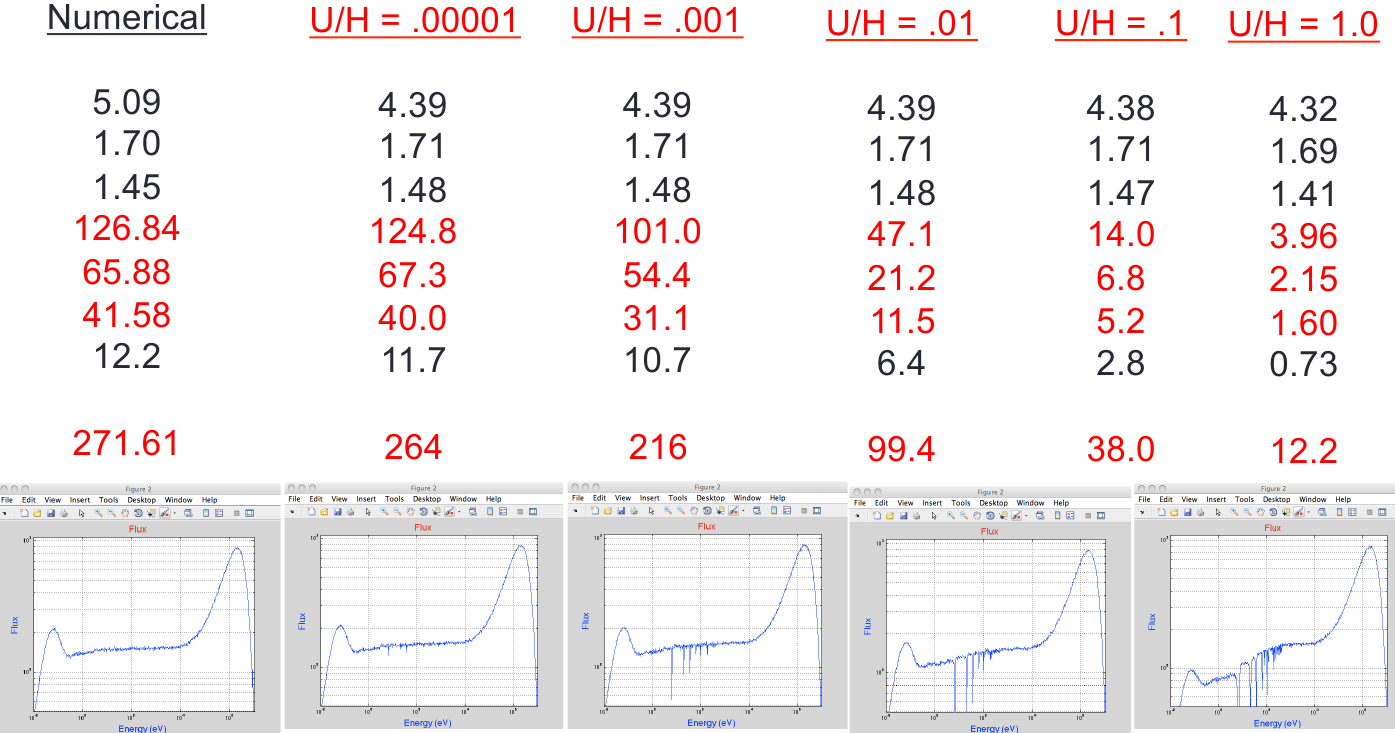
\includegraphics[width=4.5in]{images/r-m/self-shielding.png}
  \caption{Impact of Energy Self-Shielding On Effective RI} \label{energy-self-shielding}
\end{figure}



\clearpage
%%%%%%%%%%%%%%%%%%%%% SPECTRAL HARDENING %%%%%%%%%%%%%%%%%%
\topic{Spectral Hardening Shifts Resonant Absorption Rates}\label{spectral-hardening-section}
\textbf{As U/H increases, the higher energy ranges become more important, and the peak of the thermal spectrum shifts to the right. Distribution of group-wise absorption shifts towards the higher energy. $1/v$ absorption of U238 becomes more significant. Self-shielding reduces the large resonance absorption fractions. } See Figure~\ref{spectral-hardening}. 
\begin{figure}[ht]
  \centering
  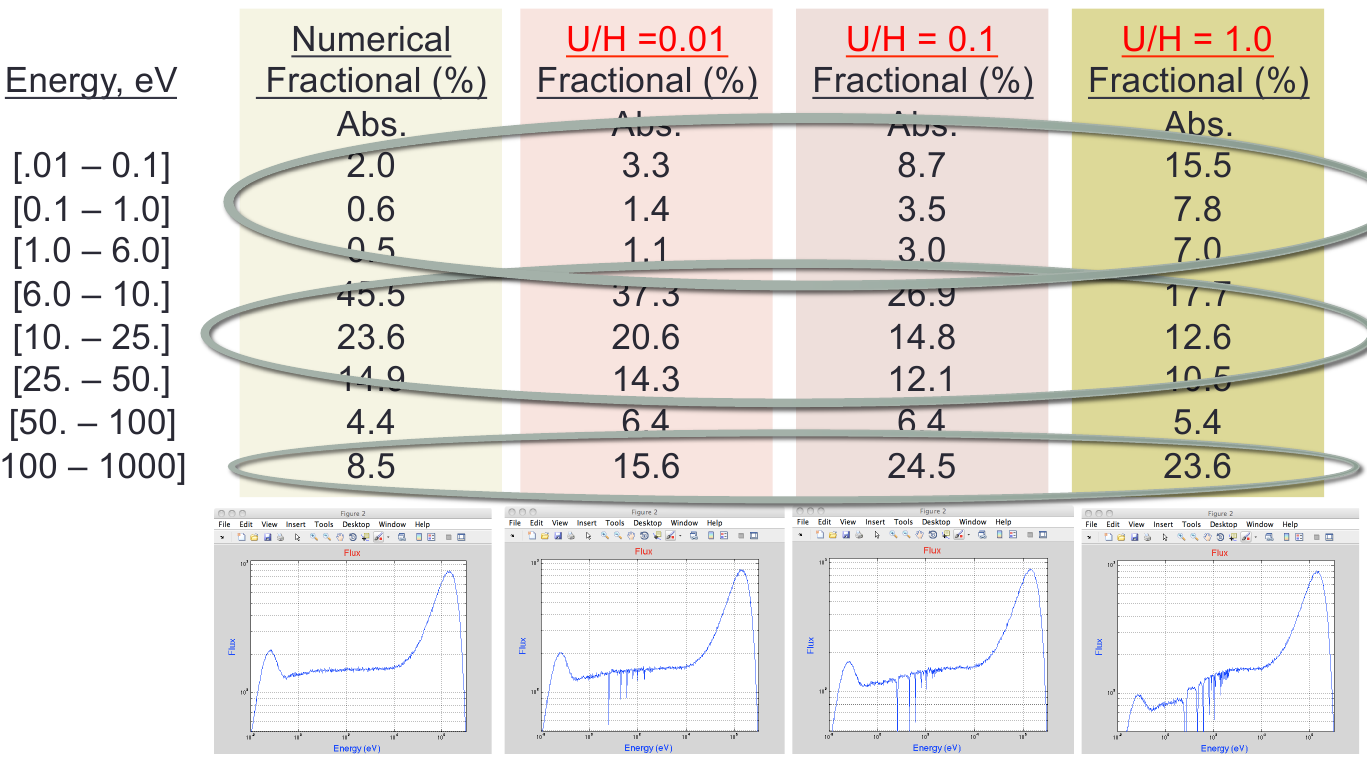
\includegraphics[width=4in]{images/r-m/spectral-hardening.png}
  \caption{Impact of Spectral Hardening On RI} \label{spectral-hardening}
\end{figure}

``As the temperature of the core material increases, the thermal neutrons maintain a Maxwellian energy distribution one but shifted increasingly towards higher energies. The thermal spectrum is said to harden. If all the cross sections in the core
had exactly a 1/v dependence, there would be no change in the thermal-neutron
interaction rates. However, most heavy nuclides have resonances near the upper end
of the thermal energy range and their cross sections, consequently, are not exactly
1/v in the thermal energy region. For example 239Pu has a large resonance at about 0.3 eV, and, as the thermal neutrons shift in energy towards this resonance, more neutrons are absorbed by 239Pu and thus the fission rate increases, thus producing a positive reactivity feedback. By contrast, hardening the thermal neutron spectrum causes a very slight decrease in absorption by 235U. 

This hardening of the thermal neutron spectrum with increasing temperature
is taken to an extreme in the TRIGA class of reactors which use as fuel enriched 235U blended in zirconium hydride. As the fuel temperature increases, vibrating hydrogen atoms trapped in the zirconium-hydride crystal lattice can transfer some
of their vibratiorial energy (about 0.13 eV) to thermal neutrons, thereby removing
them from the thermal energy region so they are less likely to be absorbed by the
fuel. This very rapid negative reactivity feedback effect is the reason these reactors
can be operated in a pulse mode, in which a large positive reactivity is inserted into
the core by rapidly removing a control rod to make the reactor very super prompt
critical. However, the ZrH negative temperature feedback acts within a few ms to
stop the runaway chain reaction, which has increased the reactor power by many
thousands of times the initial power, and brings the reactor power back to safe
limits.'' (Shultis, p.286-297). 



\end{document}
